\documentclass[11pt]{article}
\usepackage{jeffe,handout}
%\def\rmdefault{bch} % Use Charter for main text font.


% definitions for formatting code blocks
\usepackage{listings}
\usepackage{graphicx}
\usepackage{color}
\usepackage{collcell}
\newcommand{\fwcell}[1]{\makebox[\arraystretch\normalbaselineskip]{$#1$}}


\definecolor{dkgreen}{rgb}{0,0.6,0}
\definecolor{gray}{rgb}{0.5,0.5,0.5}
\definecolor{mauve}{rgb}{0.58,0,0.82}

\lstset{frame=tb,
  language=Java,
  aboveskip=3mm,
  belowskip=3mm,
  showstringspaces=false,
  columns=flexible,
  basicstyle={\small\ttfamily},
  numbers=none,
  numberstyle=\tiny\color{gray},
  keywordstyle=\color{blue},
  commentstyle=\color{dkgreen},
  stringstyle=\color{mauve},
  breaklines=true,
  breakatwhitespace=true,
  tabsize=3
}

% end definitions for formatting code blocks

\def\BOX#1{\fbox{\vbox to #1{\vss\hbox to #1{\hss}}}}
\def\Bigbox{\BOX{0.25in}}
\def\Bigbox{\raisebox{-0.5ex}[0.25in][0pt]{\BOX{0.25in}}}

\hidesolutions

\renewcommand{\arraystretch}{2}

% =========================================================
\begin{document}

\headers{CPSC 221~~~Winter 1, 2019}{}{ CSID1: \underline{d6a2b}, CSID2: \underline{~~~~~~~~~~~~}}

\begin{center}
    \LARGE
    \textbf{HW 1}
    \\[1ex]
    \Large Due 23:59 September 13, 2019 \\
\end{center}
\LARGE
\begin{tabular}{rl}
CS ID 1: & \underline{d6a2b}\\
CS ID 2: & \underline{z0n1b}\\
\end{tabular}
\large

\textbf{Instructions:}
\begin{enumerate}
\item Do not change the problem statements we are giving you. Simply add your solutions by editing this latex document. 
\item Take as much space as you need for each problem. You'll tell us where your solutions are when you submit your paper to gradescope. 
\item Export the completed assignment as a PDF file for upload to gradescope.
\item On gradescope, upload only \textbf{one} copy per partnership. (Instructions for uploading to gradescope will be posted on the HW1 page of the course website.)
\end{enumerate}

\textbf{Academic Conduct:} 
I certify that my assignment follows the academic conduct rules for of CPSC 221 as outlined on the course website. As part of those rules, when collaborating with anyone outside my group, (1) I and my collaborators took no record but names away, and (2) after a suitable break, my group created the assignment I am submitting without help from anyone other than the course staff. \\
\newpage

\newpage
\begin{problems}
%----------------------------------------------------------------------
\item (2 points)
    Using 140 characters or less, post a synopsis of your favorite movie to the
    course piazza space under the ``HW1 tell me something!'' notice, so that
    your post is visible to everyone in the class, and tagged by \#HW1num1.
    Also, use Piazza's code-formatting tools to write a {\em private} post to
    course staff that includes at least 5 lines of code. It can be code of your
    own or from a favorite project---it doesn't even have to be syntactically
    correct---but it must be formatted as a code block in your post, and also
    include the tag \#HW1num1. (Hint: Check
    \url{http://support.piazza.com/customer/portal/articles/1774756-code-blocking}).
    Finally, please write the two post numbers corresponding to your posts here:

    \begin{table}[h]
        \begin{center}
            \begin{tabular}{|l|c|}
                \hline
                Favorite Movie Post (Public) number: & {243, 311} \\ \hline
                Formatted Code Post (Private) number: & {473, 313} \\ \hline
            \end{tabular}
        \end{center}
    \end{table}

\item (16 points) In this problem, you will be a math detective! Some of the symbols and functions may not be familiar to you, but with a little digging, reading, and observing, you'll be able to figure them out. Your task is to 
    simplify each of the following expressions as much as possible, \textbf{without
    using a calculator (either hardware or software)}. Do not approximate.
    Express all rational numbers as improper fractions.
    You may assume that $n$ is an integer greater than $1$.
%    Note that $\lg n$ is shorthand for $\log_2 n$.
    Show your work in the space provided, and write your final answer in the box.
 
    \begin{enumerate}
    % Sums of arithmetic series
        \item \begin{enumerate}
  
        		\item $3 + 6 + 9 + 12 + \dots + 3n$
                \hfill
                \begin{tabular}{|l|c|}
                    \hline
                    Answer for (\theenumii.\theenumiii): & $(3/2)n(n+1)$ \\ \hline
                \end{tabular}
                \\
                \\ We can use induction to prove $S_{n}$ = $\sum_{i=1}^n i$ = 1+...+n = n(n+1)/2
                \\ Base case where n=1:
                \\ LHS: 1 = 1
                \\ RHS: 1(1+1)/2 = 1
                \\ For inductive hypothesis, assuming n=n case is true. 
                \\ For inductive step, ie n=n+1 case:
                \\ LHS: 1+...+n+n+1 = $S_{n}$+(n+1)
                \\ RHS: (n+1)(n+2)/2 = (1/2)((n+1)n+(n+1)2) = $S_{n}$+(2n+2)/2 = $S_{n}$+(n+1)
                \\ Therefore, we have proved $\sum_{i=1}^n i$ = 1+...+n = n(n+1)/2 is true.
                \\
                \\ Therefore we can say that:
                \\ $= 3+...+3n$
                \\ $= 3(1+...+n) $
                \\ $= (3/2)n(n+1)$
                \\
               \item $\displaystyle\sum_{i=1}^n (3 + 4i)$
                \hfill
                \begin{tabular}{|l|c|}
                    \hline
                    Answer for (\theenumii.\theenumiii): & $n(2n+5)$ \\ \hline
                \end{tabular}
                \\
                \\$ = \sum_{i=1}^n 3 + 4\sum_{i=1}^n i$
                \\$ = 3n + 4(n(n+1)/2)$
                \\$ = n(2n+5)$
                \vfill

               \end{enumerate}

\newpage

    % Sums of geometric series
        \item \begin{enumerate}
                \item $\displaystyle\sum_{r=2}^\infty\left(\frac{3}{5}\right)^r$
                \hfill
                \begin{tabular}{|l|c|}
                    \hline
                    Answer for (\theenumii.\theenumiii): & $\displaystyle{\frac{9}{10}}$ \\ \hline
                \end{tabular}
                \\ 
                \\We can prove that $S_{n} =  \sum_{r=0}^n\left(a\right)^r = a^{0}+...+a^{n}$, by saying that:
                \\$aS_{n} = a^{1}+...a^{n+1}$
                \\$aS_{n}-S_{n} = a^{n+1} - a^{0}$
                \\$S_{n} = (a^{n+1} - 1)/(a-1)$
                \\
                \\Additionally, if n = $\infty$, and a is less than 1, we can take the limit of the summation to infinity to solve:
                \\$=lim_{n->\infty}S_{n}$
                \\$=lim_{n->\infty}S_{n}$
                \\$=lim_{n->\infty}(a^{n+1} - 1)/(a-1)$
                \\$=-1/(a-1)$
                \\$=1/(1-a)$
                \\
                \\Therefore we can say that:
                \\$= \sum_{r=2}^\infty\left(\frac{3}{5}\right)^r$
                \\$= \sum_{r=0}^\infty\left(\frac{3}{5}\right)^r - (\frac{3}{5})^0 - (\frac{3}{5})^1 $
                \\$= -1/(\frac{3}{5}-1) - (\frac{3}{5})^0 - (\frac{3}{5})^1 $
                \\$= \frac{5}{2} - \frac{8}{5} $
                \\$= \frac{9}{10}$
                \vfill

        		\item $\displaystyle\sum_{r=(-2)}^n\left(\frac{1}{n}\right)^r$
                \hfill
                \begin{tabular}{|l|c|}
                    \hline
                    Answer for (\theenumii.\theenumiii): & $\displaystyle{\displaystyle\frac{n^{-n} + n^3 - 2n}{1-n}}$ \\ \hline
                \end{tabular}
                \\ 
                \\ $=\sum_{r=(-2)}^n\left(\frac{1}{n}\right)^r$
                \\ $=\sum_{r=0}^n\left(\frac{1}{n}\right)^r + (\frac{1}{n})^{-2} + (\frac{1}{n})^{-1} $
                \\ $=((\frac{1}{n})^{n+1} - 1)/(\frac{1}{n}-1) + (\frac{1}{n})^{-2} + (\frac{1}{n})^{-1} $
                \\ $=(n^{(-n-1)} - 1)/(\frac{1-n}{n}) + n^{2} + n $
                \\ $=\displaystyle\frac{n^{-n} - n}{1-n} + n^{2} + n $
                \\ $=\displaystyle\frac{n^{-n} + n^3 - 2n}{1-n}$
                
                \vfill
                
                \end{enumerate}
                
                \newpage
    % Sum that arises in calculating running time of heapify.
        \item \begin{enumerate}\item $\displaystyle\sum_{k=1}^{n} k2^{n-k}$
                \hfill
                \begin{tabular}{|l|c|}
                    \hline
                    Answer for (\theenumii.\theenumiii): & $\displaystyle {2^n -(3+\frac{n}{2})}$ \\ \hline
                \end{tabular}
                \\ 
                \\Say $S_{n} = \sum_{k=1}^{n} \displaystyle\frac{k}{2^k}$, we can use a proof method similar to b.i to simplify:
                \\$S_{n}=\frac{1}{2^1}+\frac{2}{2^2}...+\frac{n}{2^n}$
                \\$S_{n}/2 = \frac{1}{2^2}+\frac{2}{2^3}...+\frac{n}{2^{n+1}}$
                \\$S_{n}-S_{n}/2=(\frac{1}{2^1}+\frac{2}{2^2}...+\frac{n}{2^n})-(\frac{1}{2^2}+\frac{2}{2^3}...+\frac{n}{2^{n+1}})$
                \\$S_{n}-S_{n}/2=\sum_{i=2}^{n-1}(\frac{1}{2})^i + \frac{1}{2} - \frac{n}{2^{n+1}}$
                \\$S_{n}-S_{n}/2=\sum_{i=0}^{n}(\frac{1}{2})^i - (\frac{1}{2})^n -(\frac{1}{2})^0 -(\frac{1}{2})^1 + \frac{1}{2} - \frac{n}{2^{n+1}}$
                \\Using the equation derived in b.i, we can say that $\sum_{i=0}^{n}(\frac{1}{2})^i = \displaystyle\frac{\frac{1}{2}^{n+1} - 1}{\frac{1}{2}-1}$, and further simplify:
                \\$S_{n}-S_{n}/2=\displaystyle\frac{\frac{1}{2}^{n+1} - 1}{\frac{1}{2}-1} - (\frac{1}{2})^n -(\frac{1}{2})^0 -(\frac{1}{2})^1 + \frac{1}{2} - \frac{n}{2^{n+1}}$
                \\$S_{n}=\displaystyle 2 (\frac{\frac{1}{2}^{n+1} - 1}{\frac{1}{2}-1} - (\frac{1}{2})^n -(\frac{1}{2})^0 -(\frac{1}{2})^1 + \frac{1}{2} - \frac{n}{2^{n+1}})$
                \\$S_{n}=\displaystyle 2 (-(\frac{1}{2})^{n+1} +2 - (\frac{1}{2})^n -(\frac{1}{2})^0 -(\frac{1}{2})^1 + \frac{1}{2} - \frac{n}{2^{n+1}})$
                \\$S_{n}=\displaystyle 1-(3+\frac{n}{2})(\frac{1}{2})^n$
                \\
                \\Therefore, we can solve this question as:
                \\$=\sum_{k=1}^{n} k2^{n-k}$
                \\$=\sum_{k=1}^{n} k\displaystyle\frac{2^{n}}{2^k}$
                \\$=2^n (\displaystyle 1-(3+\frac{n}{2})(\frac{1}{2})^n)$
                \\$=2^n -(3+\frac{n}{2})$
                \\

%        \newpage
        \vfill
        
        \item $\displaystyle\prod_{k=0}^{n} (1+a^{2^k})$ \hspace{1cm} (Hint: Try multiplying by $(1-a)$.)\\
        \vspace{0.25in}
         
                \hfill \begin{tabular}{|l|c|}
                    \hline
                    Answer for (\theenumii.\theenumiii): & $\displaystyle{(1-a^{2^{n+1}})/(1-a)} $\\ \hline
                \end{tabular}
                \\ We can use induction to prove that $\displaystyle\prod_{k=0}^{n} (1+a^{2^k}) = (1-a^{2^{n+1}})/(1-a)$
                \\For base case where n = 0:
                \\ LHS: $\prod_{k=0}^{0} (1+a^{2^k}) = (1+a^{2^0}) = 1+a$
                \\ RHS: $(1-a^{2^{0+1}})/(1-a) = (1-a^2)/(1-a) = (1+a)(1-a)/(1-a) = 1+a$
                \\For induction hypothesis, we assume n=n case is true.
                \\For induction step, we prove n=n+1 case:
                \\ LHS: $\prod_{k=0}^{n+1} (1+a^{2^k}) = (1+a^{2^{n+1}})\prod_{k=0}^{n} (1+a^{2^k}) = (1+a^{2^{n+1}})(1-a^{2^{n+1}})/(1-a)$
                \\ RHS: $ (1-a^{2^{(n+1)+1}})/(1-a) = (1+a^{2^{n+1}})(1-a^{2^{n+1}})/(1-a)$
                
        \end{enumerate}
        
        \vfill     
\newpage
        \item \begin{enumerate}
        % mod
        		\item $\displaystyle7^{333} \bmod 10$
                \hfill
                \begin{tabular}{|l|c|}
                    \hline
                    Answer for (\theenumii.\theenumiii): & {7} \\ \hline
                \end{tabular}
                \\ 
                \\ $=7^{333} \bmod 10$
                \\ $=7^{4*83+1} \bmod 10$
                \\ $=((2401 \bmod 10)^{83} \bmod 10) *{7 \bmod 10}$
                \\ $=(1 \bmod 10)*{7 \bmod 10}$
                \\ = 7
                %TODO sketchy math
 
               
                \vfill
                \item $\displaystyle 16^{333} \bmod 14$
                \hfill
                \begin{tabular}{|l|c|}
                    \hline
                    Answer for (\theenumii.\theenumiii): & {8} \\ \hline
                \end{tabular}
                \\ 
                \\$= 16^{333} \bmod 14$
                \\$= (16 \bmod 14)^{333} \bmod 14$
                \\$= 2^{333} \bmod 14$
                \\$= 2^{9*37} \bmod 14$
                \\ $=(512 \bmod 14)^{37} \bmod 14$ 
                \\ $=8^{37} \bmod 14$ 
                \\ $=8^{3*12+1} \bmod 14$ 
                \\ $=(512 \bmod 14)^{12} \bmod 14 * (8^1 \bmod 14)$ 
                \\ $=8^{13} \bmod 14$
                \\ $=8^{3*4+1} \bmod 14$
                \\ $=(512 \bmod 14)^{4} \bmod 14 * (8^1 \bmod 14)$
                \\ $=8^{4+1} \bmod 14$
                \\ $=8^{3+2} \bmod 14$
                \\ $=(512 \bmod 14)^{1} \bmod 14 * (8^2 \bmod 14)$
                \\ $=8^{1+2} \bmod 14$
                \\ $=512 \bmod 14$
                \\ = 8
                \\
                \\ We could also notice that $8^n$ mod 14 is always 8.
                
                \\
                \vfill
                \end{enumerate}
\newpage

        \item \begin{enumerate}
        % log
        \item $\displaystyle32^{(\log_2 n)/4}$
                \hfill
                \begin{tabular}{|l|c|}
                    \hline
                    Answer for (\theenumii.\theenumiii): & {$n^{5/4}$} \\ \hline
                \end{tabular}
                \\ 
                \\ $=32^{(\log_2 n)/4}$
                \\ $=2^{5(\log_2 n)/4}$
                \\ $=n^{5/4}$
                \vfill

        \item $\displaystyle\frac{\log_{512} n}{\log_{2} n}$
                \hfill
                \begin{tabular}{|l|c|}
                    \hline
                    Answer for (\theenumii.\theenumiii): & {1/9} \\ \hline
                \end{tabular}
                \\ 
                \\$=\displaystyle\frac{\log_{512} n}{\log_{2} n}$
                \\$=\displaystyle\frac{\frac{\log_{2} n}{\log_{2} 512}}{\log_{2} n}$
                \\$=\displaystyle\frac{1}{\log_{2} 512}$
                \\= 1/9
                
                
                \vfill
    \end{enumerate}\end{enumerate}
\newpage


\item (9 points)
\begin{enumerate}
     \item (2 points) Fill in the blanks:
     
     Theorem: For any $c\in$  $\underline{\mathbb{Z}}$, and for any $n\in$ $\underline{2^m, m \in \mathbb{Z^{+}}}$, there exists a $k\in\mathbb{Z}$ so that $\displaystyle c^n-1 = k\cdot(c-1)$.
     \\

    \item (3 points) Prove the theorem from the previous part.
    \\
    \\We'll use induction to prove this:
    \\
    \\Base case where m = 0, n = $2^0$ = 1:
    \\LHS = $c^n-1 = c^1-1 = 0$
    \\RHS = $k\cdot(c-1) = k\cdot(1-1) = k\cdot0$
    \\Since any number multiplied by 0 is 0, k can be any number, thus there exist at least one k where it is an integer.
    \\
    \\As induction hypothesis, we'll assume that $\displaystyle A_{tru} = c^{n_{tru}}-1 = k_{tru}\cdot(c-1)$ is always true for m = m, n = $2^m$ case.
    \\
    \\ For inductive step, we'll say $m_{ind} = m_{tru}+1, n_{ind} = 2^{m_{ind}} = 2^{m_{tru}+1}$. From this, we can simplify the LHS:
    \\LHS = $\displaystyle c^{n_{ind}}-1 = c^{2^{m_{tru}+1}}-1= (c^{2^{m_{tru}}}+1)(c^{2^{m_{tru}}}-1) = (c^{2^{m_{tru}}}+1)A_{tru}$
    \\ Then, we can equate LHS and RHS to isolate $k_{ind}$ as:
    \\ $k_{ind} = (c^{2^{m_{tru}}}+1)A_{tru}/(c-1) = (c^{2^{m_{tru}}}+1)k_{tru}$
    \\
    \\ Since we know that $c, k_{tru}, m_{tru}$ are integers, we can say that $k_{ind}$ has to be integer since any integer multiplied, added, or powered by any integer always result in an integer.
    \\$\boxed{}$
    \\
    \item (4 points) Prove that $\displaystyle 5^n\cdot2^{2n} - 1$ is divisible by $19$.
    \\
    \\Before proving this, we first have to constrain n as any positive integer, since integer (such as 5 and 2) are not guaranteed to result in an integer if powered by a fraction or a negative number. 
    \\\\We can simplify the statement further by simplifying the equation:
\\$= 5^n\cdot2^{2n} - 1 $\\$= 5^n\cdot2^{2^{n}} - 1 $\\$= 5^n\cdot4^n - 1 $\\$= 20^n - 1$ 
    \\Therefore, the statement we're trying to prove is:
    \\
    \\$\forall n \in \mathbb{Z}^{+}, (20^n - 1)\mod19 = 0$
    \\
    \\ After this constraint, we can use induction to prove this:
    \\
    \\Base case, where n = 0:
\\$= 20^n - 1 $\\$= 20^0 - 1 $\\$= 1 - 1 $\\$= 0$
\\0 mod anything is 0, therefore the statement is true for base case.
\\
\\For induction hypothesis, we'll assume that for $A_{tru} = 20^{n_{tru}} - 1$, $A_{tru} \mod 19 = 0$ is always true for $n = n_{tru}$.
\\
\\For induction step, we'll say that $n = n_{ind} = n_{tru} + 1$. We can substitute $n_{ind}$ into the equation and simplify as:
\\$= 20^n - 1 $\\$= 20^{n_{ind}} - 1 $\\$= 20^{n_{tru}+1} - 1 $\\$= 20\cdot20^{n_{tru}} - 1 $\\$= (19+1)\cdot20^{n_{tru}} - 1 $\\$= (19\cdot20^{n_{tru}}) + (20^{n_{tru}} - 1) $\\$= 19\cdot20^{n_{tru}} + A_{tru}$
\\
\\ Since we know that any term that is a multiple of 19 will result in 0 if we apply mod 19, the first term of the equation will return 0 is mod 19 is applied. Since we assumed that $A_{tru}$ will return 0 if mod 19 is applied, we can say that the second term of the equation will also return 0 is mod 19 is applied. As a property of mod operation, if the sum of mod result of additive terms is less than the mod divisor, then the mod result of sum of the two additive terms is equals to the sum of mod result of additive terms. 
\\
\\Therefore, we can say that $19\cdot20^{n_{tru}} + A_{tru} = 0$, since $19\cdot20^{n_{tru}} = 0$ and $A_{tru} = 0$, prove the inductive step, and conclude that the statement is true.
\\
\\\boxed{}
    
\end{enumerate}
    \vfill\vfill
\newpage



\item  (12 points)
    \begin{enumerate}
        \item (3 points) Complete the 5-by-5 magic square below so that every row, every column, and every diagonal have the same sum, and so that each integer from 1 through 25 is used exactly once.
        
        \renewcommand{\arraystretch}{2}%
\begin{tabular}{ | *{5}{>{\collectcell\fwcell}c<{\endcollectcell} |} }
  \hline
  {19} & {25} & 8 & 11 & {2}\\
  \hline
  {13} & {1} & 17 & 24 & 10 \\
  \hline
  22 & 9 & {15} & {3} & {16} \\
  \hline
  {5} & 18 & {21} & 7 & 14 \\
  \hline
  {6} & 12 & {4} & {20} & 23 \\
  \hline
\end{tabular}
\\
        \item (3 points) Give an expression for the column sum of an $n$-by-$n$ magic square.
        
        \hfill
                \begin{tabular}{|l|c|}
                    \hline
                    Answer for (\theenumii): & ${n(1+n^2)/2}$ \\ \hline
                \end{tabular}
                \\
        \item (3 points) Consider an arrangement of the positive integers, grouped as shown, so 
        that the $k$th group has $k$ elements: $(1),(2,3),(4,5,6),(7,8,9,10), \ldots$. Find 
        a formula for the sum of the $k$ numbers in the $k$th group.
        
        \hfill
                \begin{tabular}{|l|c|}
                    \hline
                    Answer for (\theenumii): & ${k(1+k^2)/2}$ \\ \hline
                \end{tabular}
                \\
        \item (3 points) Prove that your formula from the previous part is correct. 
        \hfill
        \\
        \\We define x as the mean of the set A, which has [1...$k^2$]. If we overlay k-th group numbers on A, we can conveniently notice that (observation 0) all the numbers in a k-th group belongs in set A in the same order, and centered inside A. I arbitrarily pick 3 and 4 as sample odd and even numbers to illustrate this property. 
        \\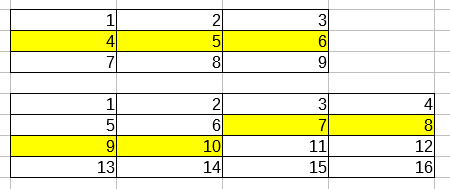
\includegraphics[]{5d.PNG}
        \\
        \\We can notice that (observation 1) if any pair of numbers is symmetric about a number, the mean of those two numbers is the original number. For example, 4 and 6 is symmetric about 5, since 4 is 1 less than 5 and 6 is 1 more than 5. This is the definition of central tendency. We also notice that (observation 2) a mean of any number is itself. For example, mean of 5 is 5. We also notice that (observation 3) if any number of sets has the same mean, the mean of the sum of the sets are the same as the individual means. For example, mean of (7,10) and mean of (8,9) is 8.5, same as mean of the individual sets.
        \\
        \\Therefore, in the case where k is even, we can pair the min and max of that set with each other, and pick the next min and the next max until all numbers are paired. Since all pairs are symmetric about the same center (due to the set being incremental by the same amount), we can say that all their mean are the same by observation 1. We can say that the mean of the set as a whole is the same as the individual means by observation 3. Because observation 0 (k-th number set is centered inside A) is true, we can say that their mean is the same as A's, defined as x, since we can apply the same pairing technique to A.
        \\
        \\The same pairing technique can be applied to cases where k is odd, by adding a pair of itself at the center of k-th numbers set and A numbers set. The mean of that pair is itself by observation 2, therefore not altering our conclusion from the even case.
        \\
        \\We can notice that 1 and $n^2$ are symmetric about x, therefore we can define x as the mean of 1 and $n^2$ by observation 1. To put that in math:
        \\$x = (1+k^2)/2$
        \\
        \\Since the mean is a number where the sum of residual (ie member - mean) is zero, we can say that the sum of any set is a multiple of its mean and its size. In other word:
        \\$x_1-\bar{x}+...+x_k-\bar{x} = 0$
        \\$x_1+...+\bar{x} = k\bar{x}$
        \\
        \\Therefore, we can say that sum of k-th group numbers set is the multiple of its mean, x, which is also defined as $(1+k^2)/2$. Therefore, we can conclude that:
        \\Sum of k-th group = $kx  = k(1+k^2)/2$
        \\
        \\\boxed{}
        \end{enumerate}
\vfill
        

\newpage


%----------------------------------------------------------------------
\item (12 points)
    Indicate for each of the following pairs of expressions $(f(n), g(n))$,
    whether $f(n)$ is $O$, $\Omega$, or $\Theta$ of $g(n)$.  Prove your answers. Note, if you choose $O$ or $\Omega$, you must also show that the relationship is not $\Theta$. 

    \begin{enumerate}
        \item $\displaystyle f(n) = n\log n$, and $\displaystyle g(n) = 3n\log n - n\log (n^2 + 2)$.
        
                \hfill
                \begin{tabular}{|l|c|}
                    \hline
                    Answer for (\theenumii): & {$f(n) = \Theta(g(n))$} \\ \hline
                \end{tabular}
                \\
                \\To prove $f(n) = \Theta(g(n))$, we must prove $f(n) = O(g(n))$ and $f(n) = \Omega(g(n))$.
                \\
                \\ 1. To prove $f(n) = O(g(n))$, we say there is a positive c and $n_0$ such that f(n) is less than or equal to c*g(n) for all n more than or equal to $n_0$.
                \\ This case, we can pick c = 2, $n_0$ = 100.
                \\ f(n) = 100log(100) = 200
                \\c*g(n) = (3(100)log(100)-100(log(10000 + 2))*2 = 399.98
                \\Since both f(n) and g(n) tends to positive infinity from $n_0$ without any n where instantaneous speed of f(n) or g(n) equals 0, we can say that $f(n) = O(g(n))$ for this chosen c and $n_0$.
                \\
                \\or
                \\
                \\Choose c = 100 $n_0$ = 2
                \\
                \\ $nlog(n) $\leq$ 300nlog(n) - 100nlog(n^2 +2)$
                \\
                \\$0 $\leq$ 299nlog(n) - 100nlog(n^2 +2)$
                \\
                \\This will always be true because the term will always be positive for $n > 2$
                \\
        
                \\2. To prove $f(n) = \Omega(g(n))$, we say there is a positive c and $n_0$ such that f(x) is more than or equal to c*g(x) for all n more than or equal to $n_0$.
                \\This case, we can pick c = 1, $n_0$ = 100.
                \\ f(n) = 100log(100) = 200
                \\c*g(n) = 3(100)log(100)-100(log(10000 + 2) = 199.991
                \\Since both f(n) and g(n) tends to positive infinity from $n_0$ without any n where instantaneous speed of f(n) or g(n) equals 0, we can say that $f(n) = \Omega(g(n))$ for this chosen c and $n_0$.
                \\
                \\Or 
                \\Choose c = 1/3 and $n_0$ = 2
                \\ $nlog(n) $\geq$ nlog(n) - (1/3)nlog(n^2 +2)$
                \\$0 $\geq$ -(1/3)nlog(n^2 +2)$
                \\
                \\This inequality will always hold true because $-(1/3)nlog(n^2 +2)$ 
                \\will always be negative for $n $\geq$ 2$
                \\

                \\\boxed{}
                        
                \item $\displaystyle f(n) =  \frac{1}{2}n^3$, and $g(n) = n^2 + 4n + 37$.
        
                \hfill
                \begin{tabular}{|l|c|}
                    \hline
                    Answer for (\theenumii): & {$f(n) = \Omega(g(n))$} \\ \hline
                \end{tabular}
                
                
                \\
                \\To prove $f(n) = \Omega(g(n))$, we can pick c = 1, $n_0$ = 1000.
                \\ f(n) = $(1/2)*(1000^3) = 5*10^8$
                \\c*g(n) = $1000^2+4000+37 = 1.004037*10^6$
                \\Since both f(n) and g(n) tends to positive infinity from $n_0$ without any n where instantaneous speed of f(n) or g(n) equals 0, we can say that $f(n) = \Omega(g(n))$ for this chosen c and $n_0$.
                \\
                \\However, $f(n) = O(g(n))$ is not true because for any c and $n_0$ we pick, there will be n such that n is more than or equal to $n_0$ and f(n) is more than or equal to c*g(n). 
                \\To prove this, we can pick any arbitrary c and $n_0$, and pick n as $2(cn_0+6)$.
                \\1. n is always more than $n_0$ since $2(cn_0+6)$ is always more than $n_0$ where c and $n_0$ are positive real numbers.
                \\2. We can substitute n into the equations:
                \\f(n) = $(2(cn_0+6))^3/2 = 4((cn_0)^3+18(cn_0)^2+108(cn_0)+216) = 4c^3n_{0}^3+72c^2n_{0}^2+432cn_0+864$
                \\c*g(n) = $c((2(cn_0+6))^2+4(2(cn_0+6))+37) = 4c^3n_{0}^2+56c^2n_0+229c$
                \\ We can substitute f(n) and c*g(n) into the equation $f(n) \leq c*g(n)$ to check if $f(n) = O(g(n))$ is true or not:
                \\$f(n) \leq c*g(n)$
                \\$4c^3n_{0}^3+72c^2n_{0}^2+432cn_0+864 \leq 4c^3n_{0}^2+56c^2n_0+229c$
                \\Very obviously, however, we can notice that each terms of f(n) is more than or equals to each terms of c*g(n). In other words:
                \\$4c^3n_{0}^3 \geq 4c^3n_{0}^2$
                \\$72c^2n_{0}^2 \geq 56c^2n_0$
                \\$432cn_0 \geq 229c$
                \\$864 \geq 0$
                \\Therefore, the inequality is not true, and we conclusively proved that there exists n where $f(n) = O(g(n))$ is false for any c and $n_0$.
                
\\\boxed{}
                
\vfill                
          \end{enumerate}
\newpage

 
\item (16 points)
  For each C++ function below, give the tightest asymptotic upper bound that you can determine for the function's {\bf runtime}, in terms of the input parameter. Where prompted, also compute the return value of the function.  Express both runtime and return value in simplest terms.
  For all function calls, assume that the input parameter $n \geq 1$.
  
  \begin{enumerate}
  
  \item
    \begin{lstlisting}
int coffee(int n) {
   int s = n * n;
   for (int q = 0; q < n; q++)
      s = s - q;
   for (int q = n; q > 0; q--)
      s = s - q;
   return s + 2;
}
\end{lstlisting}

\vfill

    \hfill
    \begin{tabular}{|l|c|}
      \hline
      Return value for (\theenumii): & {2} \\ \hline
    \end{tabular}
    

\hfill
\begin{tabular}{|l|c|}
      \hline
     Running time of (\theenumii): & {O(n)} \\ \hline
    \end{tabular}
    \vskip 0.5in
  \item
    \begin{lstlisting}
	int tea(int n) {
		int r = 0;
		for (int i = 1; i < n*n*n; i = i * 2)
  		    r++;
  		return r * r;
	}
    \end{lstlisting}
    
    \hfill
    \begin{tabular}{|l|c|}
      \hline
      Return value for (\theenumii): &
      ${\ceil{log_2(n^3)}^2}$ \\ \hline
    \end{tabular}
        \vskip 0.5in

\hfill
\begin{tabular}{|l|c|}
      \hline
     Running time of (\theenumii): & ${O(log(n))}$ \\ \hline
    \end{tabular}
    \vskip 0.5in
  \newpage
  \item
    \begin{lstlisting}
	int mocha(int n) {
  		int r = 0;
  		for (int i=0; i<=n; i = i+16)
  		    for (int j=0; j<i; j++)
  		        r++;
  		return r;
	}
    \end{lstlisting}
    
    
    \hfill
    \begin{tabular}{|l|c|}
      \hline
      Return value for (\theenumii): & ${8\cdot\floor{n/16}\cdot(\floor{n/16}+1)}$ \\ \hline
    \end{tabular}
%        \vskip 0.5in

\hfill
\begin{tabular}{|l|c|}
      \hline
     Running time of (\theenumii): & ${O(n^2)}$ \\ \hline
    \end{tabular}
    \vskip 0.5in

  
  \item
    \begin{lstlisting}
	int espresso(int n) {
	    int j=0;
  		for (int k = 16; coffee(k) * mocha(k) - k <= n; k+=16) {
  		    j++;
    		cout << "I am having so much fun with asymptotics!" << endl;
    	}
	    return j;
	}
    \end{lstlisting}

\hfill
    \begin{tabular}{|l|c|}
      \hline
      Return value for (\theenumii): & ${\floor{\sqrt{n/16}}}$ \\ \hline
    \end{tabular}
 %       \vskip 0.5in

\hfill
    \begin{tabular}{|l|c|}
      \hline
      Running time of (\theenumii): & ${O(n^3)}$ \\ \hline
    \end{tabular}
        \vskip 0.5in

    
\newpage

  \item
    \begin{lstlisting}
	int latte(int n) {
	    int j = 0;
	    for (int k = 0; k < coffee(k) * n; k++)
	        j = j + 2;
  		return espresso(mocha(j));
	}
    \end{lstlisting}

    \hfill
    \begin{tabular}{|l|c|}
      \hline
      Running time of (\theenumii): & ${O(n^3)}$ \\ \hline
    \end{tabular}
        \vskip 0.5in


  
  \end{enumerate}


\end{problems}

\newpage
%----------------------------------------------------------------------
Blank sheet for extra work.

\end{document}
